\chapter{Specification}
\label{ch:specification}
The presented system requests pages from card market website and scrapes their content to build a knowledge database helping the user take better decisions as a buyer. The results are presented in a form of a simple web application, as presented on Fig. \ref{fig:web_app} and \ref{fig:web_app_best_set_seller}, as well as in the form of graphs and plots in the \textit{analysis} directory.

\begin{figure}
    \centering
    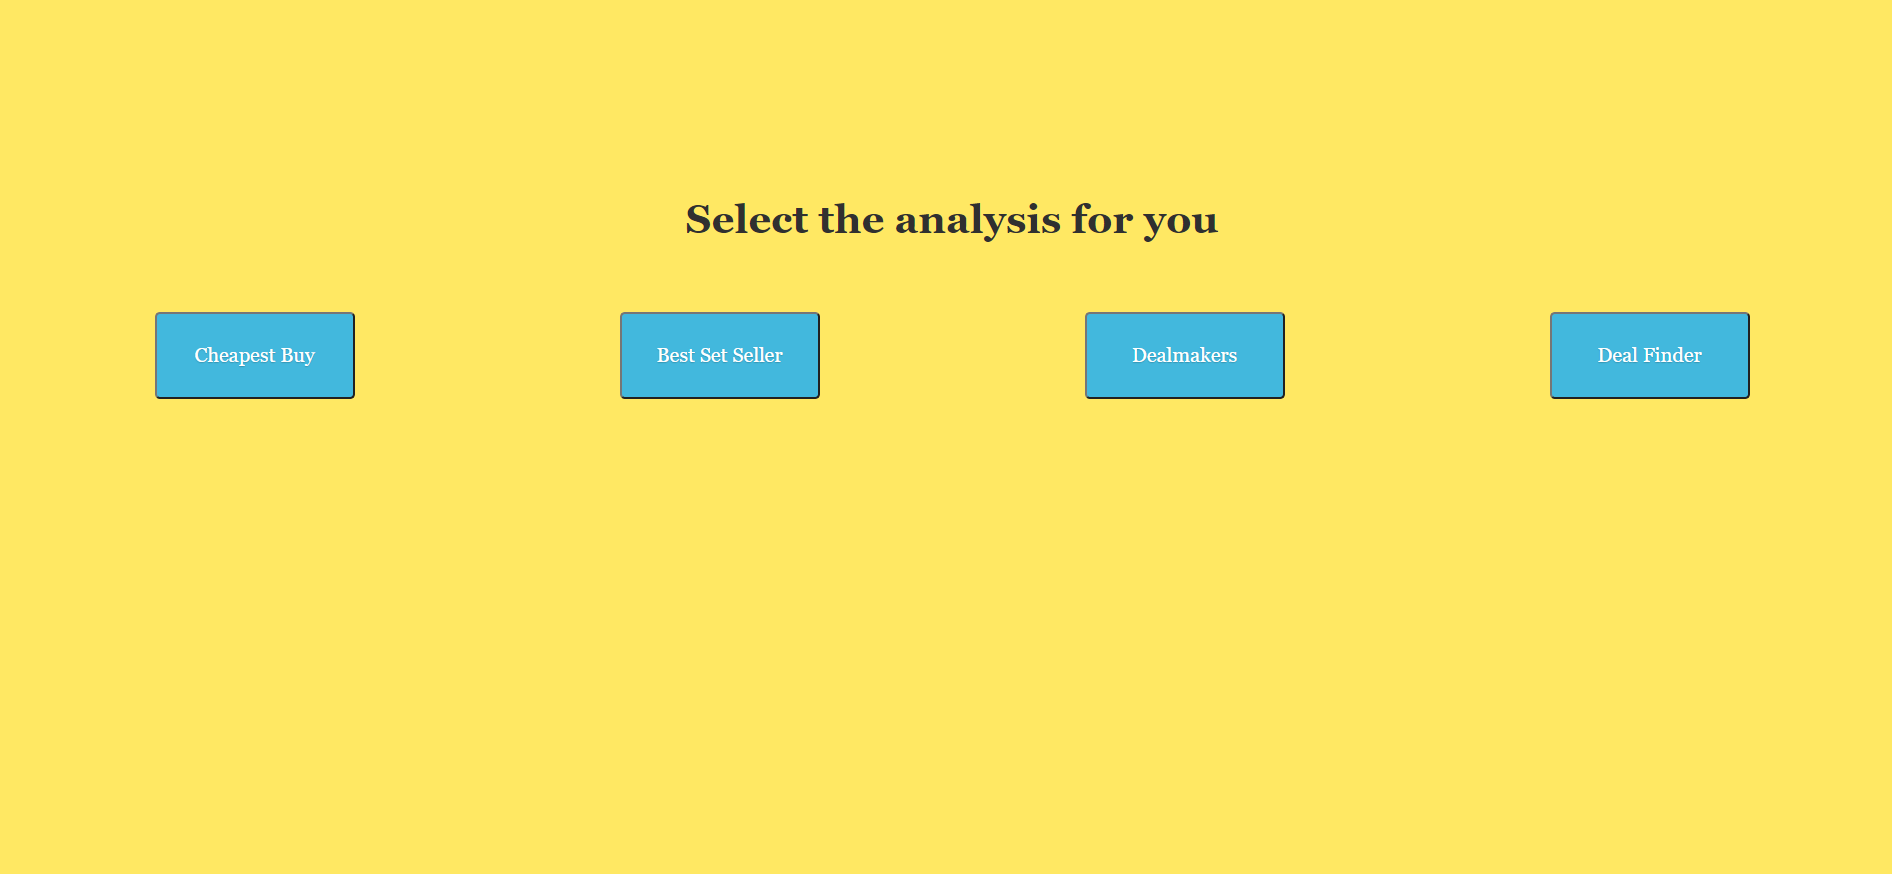
\includegraphics[width=\textwidth]{figures/web_app.png}
    \caption{Simple web interface for performing analysis}
    \label{fig:web_app}
\end{figure}

\begin{figure}
    \centering
    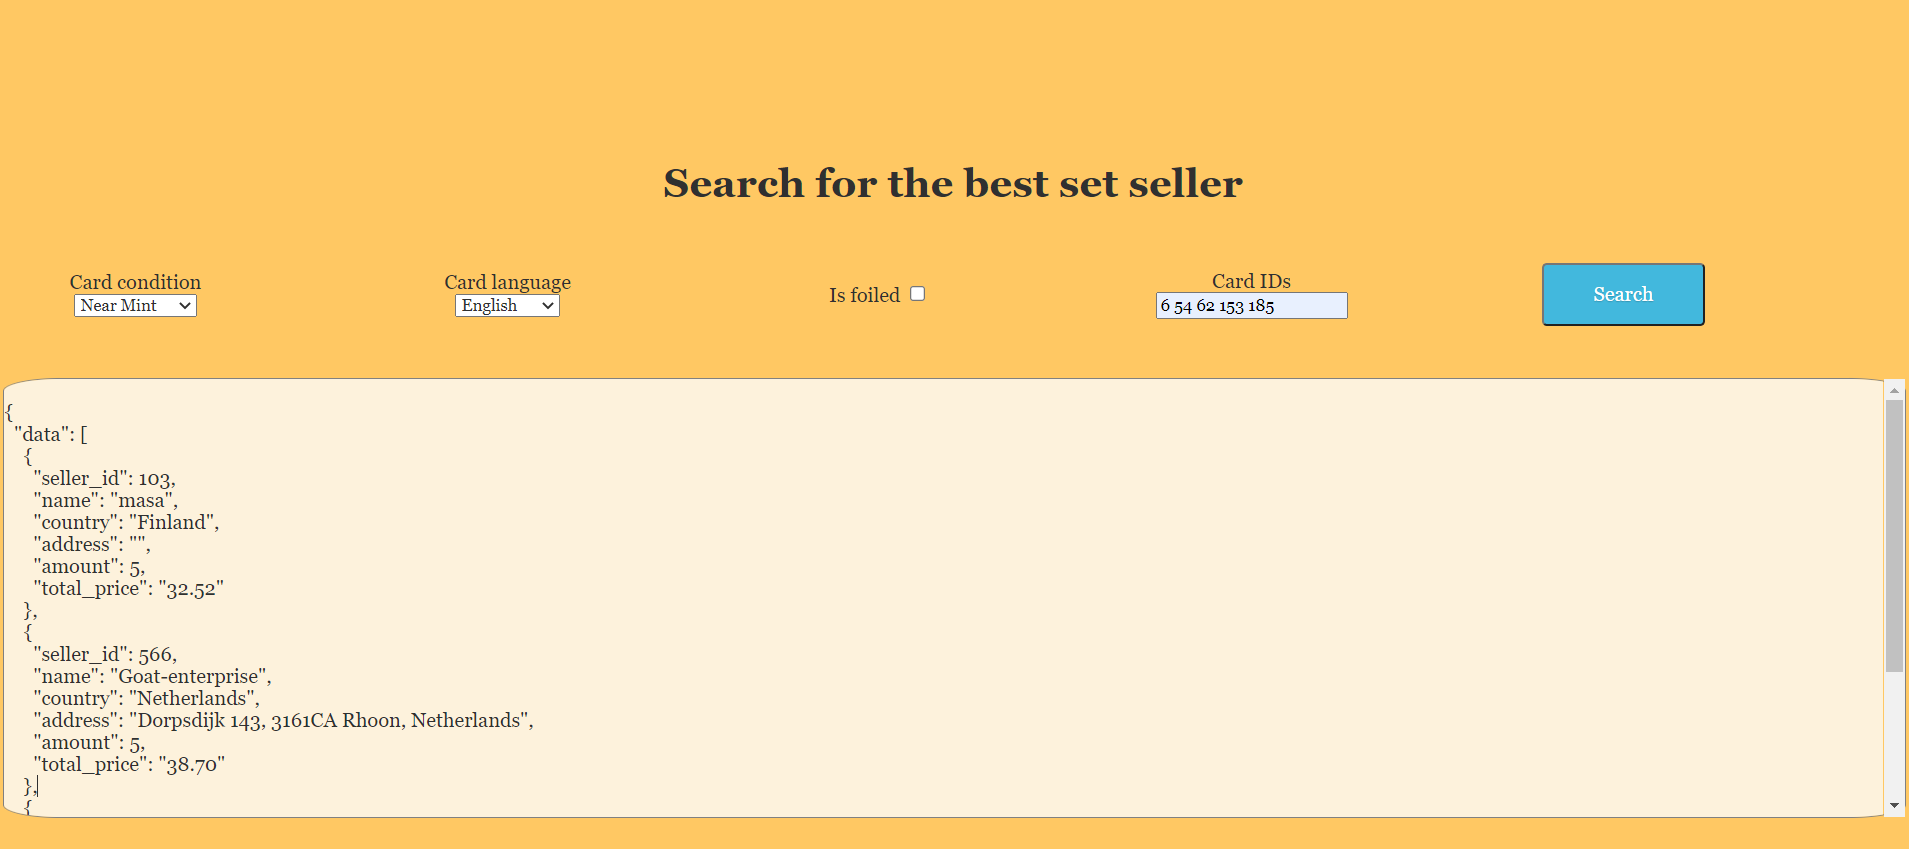
\includegraphics[width=\textwidth]{figures/web_app_best_set_seller.png}
    \caption{Searching for the user selling a batch of cards with given conditions}
    \label{fig:web_app_best_set_seller}
\end{figure}

Implementation of the thesis topic involves a containerization software --- \textit{Docker} --- which hosts several subapplications written as semi-standalone scripts, each responsible for a part of the data pipeline. Using Python and its vast collection of libraries the author is handling the data scraping, intial cleaning and maintenance of the pre-stage database in compressed CSV files; as well as managing the MySQL database, creating helper tables, extracting new information and visualizing the data to answer user's questions. With JavaScript, SQL and HTML the web application is querying the database connected to a \textit{Node.js} server.


\section{Functional requirements}
The system is required to do the following:
\begin{enumerate}
    \item The system should gather cards, sellers and offers' data and keep it up to date
    \item The system should allow the user to choose an expansion of cards to gather
    \item The data gathering system should run continuously and gather data once a day
    \item The gathering system should visit all card sites from specified expansion and save (a) card information, dynamic and static, and (b) full information about sale offers of this card to CSV files
    \item The gathering system should visit profile pages of all newly-encountered sellers and save their public data to a CSV file
    \item The gathering system should keep track of the date and save the date data into a CSV file
    \item The database manager system should run continuously and update the database whenever new complete batch of data has been gathered
    \item The data miner system should run continuously and create data marts every hour, given the database has the newest data
    \item The web application should run continuously, recovering from errors and providing the user with at least four ways of getting useful information from the data
\end{enumerate}


\section{Non-functional requirements}
\begin{enumerate}
    \item The total time of data processing should be less than 6 hours
    \item The system should be standalone (bootstrapping itself from \textit{docker-compose.yml} and code), and cross-platform compatible
    \item The gathering system should adapt the requests frequency to the server condition
    \item No user input is required after running the system
\end{enumerate}


\section{Problem domain}
The main goal of this project is to optimize user's card buying decisions basing on the data gathered in the warehouse.

\subsection{Trading card games}
Trading card games (\textit{TCG}), also known as collectible card games (\textit{CCG}), are types of card games combining the elements of strategic gameplay and features of trading cards.
The first TCG was released in 1993 under the name Magic: The Gathering (\textit{MTG}). The game, released by an eight-person company, was an overnight success, with over 10 million cards sold in just 6 weeks.
Two years later, this basement business became a gaming corporation. Today, \textit{MTG} is among the most popular TCGs with roughly 35 million players as of December 2018 \cite{magicTheGathering}. \par
During the game, the goal of each player is to reduce the opponent's life points by strategically playing cards from the hand, before the other one succeeds. However, each player can compile their own deck of 60\footnote{Some variations require a deck of 40 cards, which are selected from a random pool of cards} cards out of the thousands available. This makes every gameplay unique on a level which is fundamentally different from the classic cards. One doens't have to be an expert in the field to understand that the more cards one has, especially good cards, the higher the chances of winning. Thus, trading the cards becomes an aspect as crucial as the strategy itself. \par
One of the places where \textit{MTG} cards can be bought is \url{www.cardsmarket.com/} --- an online market with a myriad of cards from the game listed for sale, by users from around the world, majority of which lives in Europe. Users are divided into three categories: \textit{Amateur}, \textit{Professional} and \textit{Powerseller}, depending on their setup and \textit{modus operandi} (individuals, zealous hobbyists, card stores). To spend the least amount of money while collecting the most wanted cards, i.e. to optimize the shopping, one would have to analyze thousands of bits of data, from the average prices of all cards, to the velocity of sales and of restocking the virtual shelves.

\subsection{Market-related entities}
\label{entities}
Each card has a name, an expansion, which is a higher-level grouping of cards, and rarity. These elements do not vary with time. However, the number of cards for sale, and automatically calculated price statistics change every day, that's why these are stored in a separate table, with new rows every day. Similarly, the seller has a name, country of residence and optionally an address, year of registration and what type of seller they are (private vs professional); while the table with sale offers stores every card offer from every seller, from each day. To add a unified time dimension to the data, a date table is created with unique \textit{date\_id} designating the day, month and year of the datapoint collection.

When the data from the card market is collected, it is stored in five CSV files and one text file. The text file, named after set expansion, contains card names in the order of first visit and it's used to maintain consistent card-to-card progression between runs. Then, each CSV file represents one entity: \textit{card}, \textit{seller} (static entities), \textit{card\_stats}, \textit{date} and \textit{sale\_offer} (dynamic entities).

\subsection{Problem formulation}
From the point of view of a card collectioner, every potential buy should be analyzed for better offers in order to minimize losses. The main goals of the user among buying needed cards at the lowest possible price, without sacrificing the various card qualities; finding the most price-slashing, discout-oriented sellers; discovering which cards are more discounted than others, and thus make a better buy opportunity; or minimizing the shipping costs by ordering a whole set of cards from a single seller, should one exist. Therefore, the main questions posed by the user should be answered accordingly:
\begin{enumerate}
    \item Given a non-empty list of card ids (and card qualities: language, condition, whether it is foiled), find three sellers that sell that card at the lowest price.
    \item Given a non-empty list of card ids (and card qualities) rank them based on price statistics, to highlight the most discounted cards.
    \item Given a non-empty list of card ids (and card qualities) select users selling the maximum amount of wanted cards, ordered by the lowest total price.
    \item Given wanted card qualities, find which sellers have a high amount of discounted cards and the biggest differences between the average market prices and their prices.
    \item Additionally, present as much novel information and insights from the data as possible.
\end{enumerate}

\section{Data warehouse modelling}
The data warehouse lifecycle beings when the data is collected. The pre-stage area encompasses what is written in the CSV files after a gathering run. These files correspond to entities from subsection (\ref{entities}) and to the tables presented below.

\subsection{Base tables}
\label{ss:base_tables}
After the data is gathered from the website, and stored in the CSV files, the database manager updates an image-based MySQL server running in Docker, creating the tables corresponding to each entity (seen in Fig. \ref{fig:database})--- and data miner adds new tables as data marts for future use, and performs other analyses and visualizations.

\begin{figure}[ht]
    \centering
    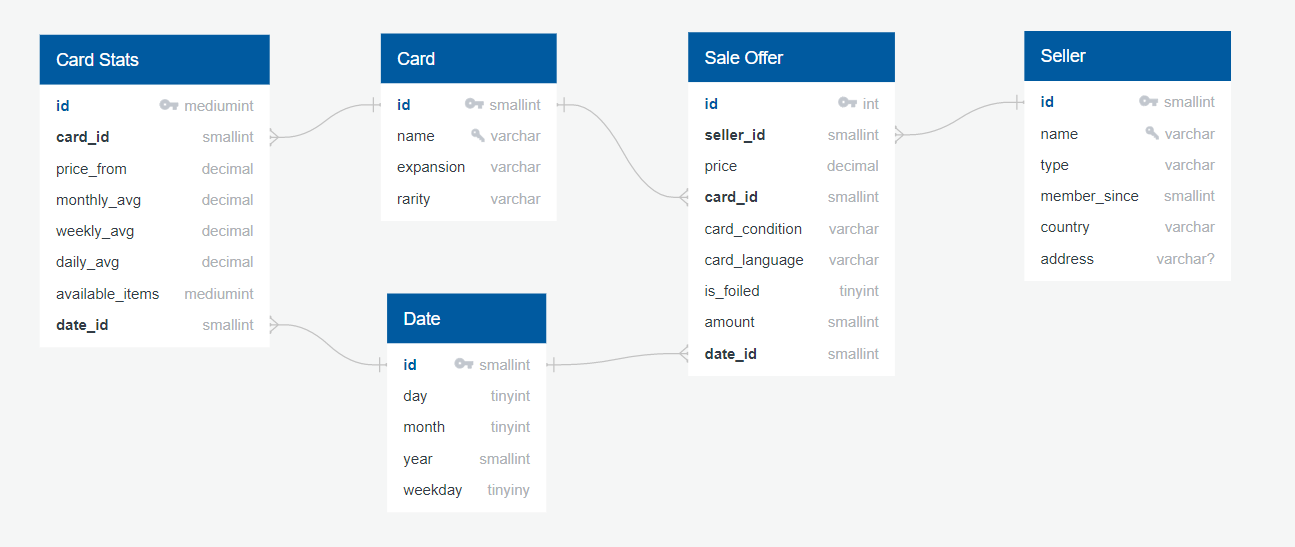
\includegraphics[width=\textwidth]{figures/database.png}
    \caption{Database schema with the five base tables}
    \label{fig:database}
\end{figure}

\subsection{Helper tables}
The data miner creates new tables basing on the five elemental ones, in order to speed up the processing of SQL queries. The largest and most problematic table is the \textit{sale\_offer} with few millions of records, eight attributes each. To reduce the loading time, the newest day is selected as a separate table. Similarly, last two weeks are another temporal subset, extraction of which helps with performance.

\section{Containers overview}
The task of the \textit{firefox\_webdriver} container is to provide a constant and reliable access to a browser-like solution for an automated page navigation.

The \textit{mysql\_database} container hosts a database with persistent memory, storing the major part of the data warehouse and making it accessible to other containers.

The \textit{data\_gathering} subsystem automatically scrapes and collects the web data in the \textit{data} directory, while \textit{database\_manager} takes this data and passes it to the database. It is important for the \textit{database\_manager} to be slightly delayed with respect to \textit{data\_gathering}, for reasons that are explained in section (\ref{container_orchestration}).

The \textit{data\_miner} and \textit{node\_server} containers are dependent only on the database, however here boot order and system state are not as important; these asynchonous containers perform their job properly when the data is ready and don't cause critial failure when it's not, which is enough for the application to run reliably.

The \textit{node\_server} container hosts a website served by a Node.js server, that presents the user with four functional analyses of the card market.

Each container has its own virtual storage, so to perform tasks on a shared set of data, both docker volumes and data mounts are introduced. Additionally, each container exposes one port internally to a port on the host, inside a network encompassing the whole solution.
